\newpage
\subsection{UC3 - Modifica dei Metadati}
\label{subsec:uc3}

\begin{figure}[h]
    \centering
    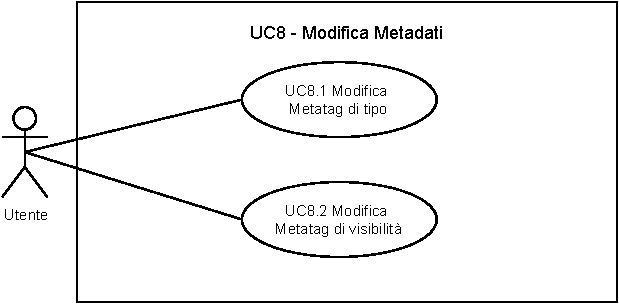
\includegraphics[width=0.7\textwidth]{componenti/casi-duso/diagrammi/UC3.pdf}
    \caption{Diagramma rappresentante UC3}
    \label{fig:UC3}
\end{figure}

%TODO: Al posto di cosi fare cosà:
        % Utente vuole modificare i metadati relativi ad una dimensione.
        % UTente sceglie dimensione. 
        % Utente modifca i metadati che preferisce.
\begin{itemize}
    \item \textbf{Descrizione}: L’utente vuole modificare un metadato attualmente assegnati ad una dimensione del dataset.
	
    \item \textbf{Attore primario}: Utente.
    
    \item \textbf{Precondizione}:   Nel programma è stato importato un dataset dotato di metadati per ogni sua dimensione.
    \item \textbf{Postcondizione}:  Vengono aggiornati i metadati della dimensione scelta dall'utente.

	\item \textbf{Scenario principale}:
        \begin{enumerate}
                \item L'utente sceglie una dimensione da modificare.
                \item L'utente esegue le modifiche che preferisce tra quelle rese possibili.
                \item L'utente valida le modifiche apportate selezionando un pulsante di "conferma"
        \end{enumerate}
    
    \item \textbf{Scenario alternativo}:
		\begin{enumerate}
			\item L'utente decide di annullare le modifiche selezionando il pulsante "annulla".
			\item Vengono ripristinati i metadati della dimensione precedenti alla modifica.
        \end{enumerate}
\end{itemize}

\newpage
\subsubsection{UC3.1 - Modifica metadato di tipo}
\label{subsubsec:uc3.1}

\begin{itemize}
    \item \textbf{Descrizione}: L’utente vuole modificare il metadato di tipo attualmente assegnato 
                                alla dimensione del dataset da lui selezionata. Egli sceglie il nuovo valore le opzioni che gli vengono rese disponibili.
	
    \item \textbf{Attore primario}: Utente.
    
    \item \textbf{Precondizione}:   L'utente ha selezionato una dimensione del dataset  da modificare
                                    e la voce "modifica metadato di tipo" dal menu di modifica dei metadati.
    \item \textbf{Postcondizione}:  Viene aggiornato il metadato di tipo della dimensione selezionata.

	\item \textbf{Scenario principale}:
        L'utente imposta il nuovo tipo tra le opzioni possibili per la dimensione selezionata.
\end{itemize}


\subsubsection{UC3.2 - Modifica metadato di visibilità}
\label{subsubsec:uc3.2}

\begin{itemize}
    \item \textbf{Descrizione}: L’utente vuole modificare il metadato di visibilità attualmente 
                                assegnato alla dimensione del dataset da lui scelta.
                                Egli sceglie se rendere la dimensione visibile o nascosta.
	
    \item \textbf{Attore primario}: Utente.
    
    \item \textbf{Precondizione}:   L'utente ha selezionato una dimensione del dataset da modificare
                                    e la voce "modifica metadato di visibilità" dal menu di modifica dei metadati.

    \item \textbf{Postcondizione}:  Viene aggiornato il metadato di visibilità della dimensione selezionata.

	\item \textbf{Scenario principale}: L'utente imposta la nuova impostazione di visibilità tra "visibile" e "nascosta".
\end{itemize}

